\documentclass[12pt,a4paper]{report}

% Encodage et langue
\usepackage[utf8]{inputenc}
\usepackage[T1]{fontenc}
\usepackage[french]{babel}
\usepackage[absolute,overlay]{textpos}


% Mise en page
\usepackage{geometry}
\geometry{left=2.5cm,right=2.5cm,top=2.5cm,bottom=2.5cm}
\usepackage{setspace}
\onehalfspacing

% En-têtes/pieds de page
\usepackage{fancyhdr}
\pagestyle{fancy}
\fancyhf{}
\lhead{Serpent}
\rhead{UNC - 2025}
\cfoot{\thepage}


% Maths et figures
\usepackage{amsmath, amssymb}
\usepackage{graphicx}
\usepackage{hyperref}


% Pour la bibliographie simple
\usepackage{url}

\renewcommand{\thesubsection}{\arabic{subsection}}


\begin{document}

% Page de garde
\begin{titlepage}

    % --- Logo en haut à droite ---
    \begin{textblock*}{5cm}(15cm,0.5cm)
        
\includegraphics[width=5cm]{assets/logo.png} 
    \end{textblock*}

    % --- Titre justifié et limité ---
    \noindent
    \begin{minipage}{13cm}
        \raggedright
        {\scshape\Huge \textbf{Algorithme de chiffrement par bloc : Serpent} \par}
    \end{minipage}

    \vspace{0.5cm}

    \rule{\linewidth}{0.4pt}
    
    \vspace{0.1cm}

    \centering
    {\Large Rapport\par}

    \vspace{1.5cm}
    {\large NGUYEN Alexandre - MILLOT Nathan\par}

    \vspace{4cm}
    % --- Image du sujet ---
    \begin{center}
        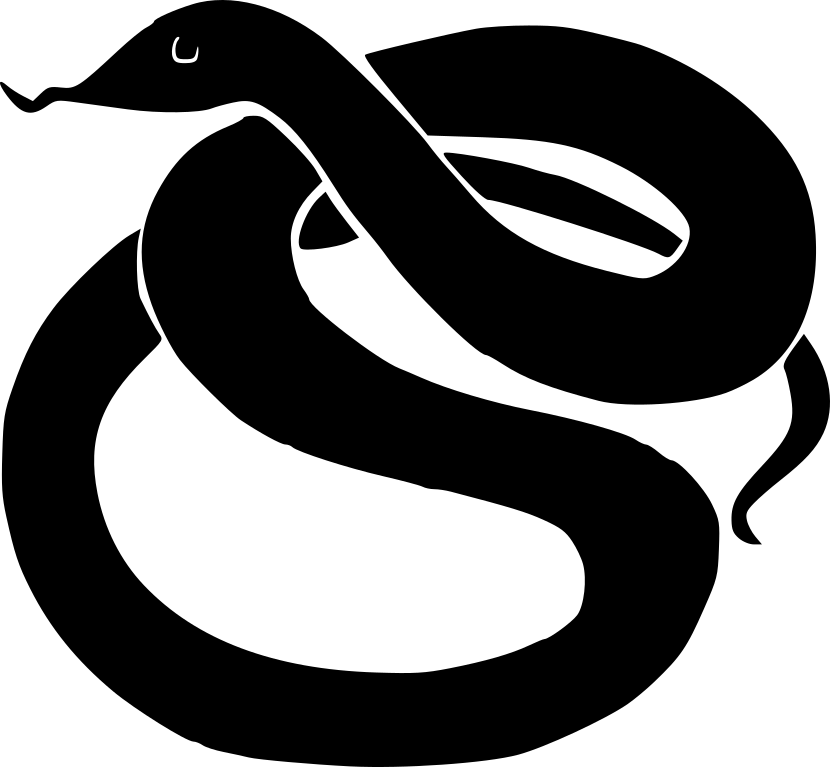
\includegraphics[width=0.5\linewidth]{assets/serpent.png}
    \end{center}

    \vspace{2.5cm}
    {\large Licence Informatique TREC 7  Semestre 6 \par}
   
    \vspace{1cm}
    {\large Date : \today \par}

\end{titlepage}

\tableofcontents

\section*{Espaces de définition}
\addcontentsline{toc}{section}{Espaces de définition}

\subsection{Messages en clair et chiffrés}
L’algorithme Serpent est un chiffrement par bloc avec :
\begin{itemize}
    \item Espace des messages en clair $M = \{0,1\}^{128}$ ;
    \item Espace des messages chiffrés $C = \{0,1\}^{128}$.
\end{itemize}
Chaque bloc est donc constitué de 128 bits.

\subsection{Clés}
L’espace des clés dépend de la taille choisie :
\begin{itemize}
    \item $K = \{0,1\}^{128}$ ;
    \item $K = \{0,1\}^{192}$ ;
    \item $K = \{0,1\}^{256}$.
\end{itemize}
En pratique, Serpent est défini pour ces trois tailles de clé.

\section*{Description du schéma Serpent}
\addcontentsline{toc}{section}{Description du schéma Serpent}

\setcounter{subsection}{0}

\subsection{Structure générale}
Serpent est basé sur un \textbf{réseau de substitution-permutation (SPN)}.  
Il comporte 32 tours successifs :
\begin{enumerate}
    \item Ajout de sous-clé (XOR avec la sous-clé de tour) ;
    \item Substitution via une des 8 S-boxes (non-linéarité) ;
    \item Transformation linéaire (permutation de bits).
\end{enumerate}

\begin{figure}[h]
    \centering
    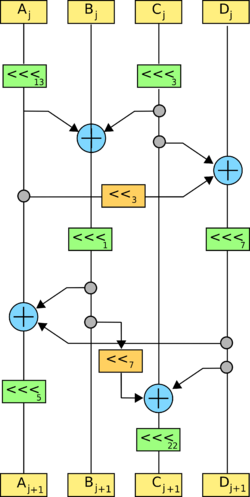
\includegraphics[width=0.35\textwidth]{assets/serpent-global.png}
    \caption{Schéma général de Serpent}
\end{figure}

\subsection{Sous-fonctions}

\subsubsection{Génération de sous-clés}
À partir de la clé initiale, Serpent dérive 33 sous-clés de 128 bits chacune, notées $K_0, K_1, \dots, K_{32}$.

\subsubsection{Substitution (S-boxes)}
Huit S-boxes différentes sont utilisées, notées $S_0, \dots, S_7$.  
Elles transforment des blocs de 4 bits en 4 bits, et sont choisies de manière cyclique au fil des tours.

\subsubsection{Transformation linéaire}
Chaque tour applique une permutation fixe des bits pour assurer une bonne diffusion.

\subsubsection{Dernier tour}
Le dernier tour est légèrement différent : après la substitution, il n’y a pas de transformation linéaire, seulement l’ajout de sous-clé.

\section*{Exemple de chiffrement simplifié}
\addcontentsline{toc}{section}{Exemple de chiffrement simplifié}

Pour illustrer le fonctionnement de l'algorithme Serpent, nous présentons un exemple simplifié avec un bloc de données réduit à 8 bits (au lieu de 128 bits) et deux tours (au lieu de 32). Cet exemple suit la structure réelle de Serpent : ajout de sous-clé, substitution via S-box, et transformation linéaire, sauf pour le dernier tour où la transformation linéaire est omise, suivie d'un XOR final avec la dernière sous-clé. Nous inclurons également le déchiffrement pour montrer comment inverser le processus. Dans la réalité, Serpent traite des blocs de 128 bits avec 32 tours complets et 33 sous-clés de 128 bits.

\subsection{Données initiales}
Prenons les données suivantes :
\begin{itemize}
    \item \textbf{Texte clair} : \( B = 10101010 \) (8 bits, équivalent à \texttt{0xAA} en hexadécimal).
    \item \textbf{Sous-clés} (simplifiées, 8 bits chacune) :
    \begin{itemize}
        \item \( K_0 = 11110000 \) (\texttt{0xF0}),
        \item \( K_1 = 10101010 \) (\texttt{0xAA}),
        \item \( K_2 = 11001100 \) (\texttt{0xCC}).
    \end{itemize}
    \item \textbf{S-boxes} : Nous utilisons deux S-boxes inspirées des \( S_0 \) et \( S_1 \) réelles de Serpent, définies pour des entrées de 4 bits (voir Tableaux~\ref{tab:sbox0} et~\ref{tab:sbox1}). Pour simplifier, seules les entrées utilisées dans l'exemple sont listées. Pour le déchiffrement, nous utilisons leurs inverses (voir Tableaux~\ref{tab:sbox0_inv} et~\ref{tab:sbox1_inv}).
\end{itemize}

\begin{table}[h]
    \centering
    \begin{tabular}{|c|c|c|c|}
        \hline
        Entrée (décimal) & Entrée (binaire) & Sortie (décimal) & Sortie (binaire) \\
        \hline
        0 & 0000 & 3 & 0011 \\
        1 & 0001 & 8 & 1000 \\
        5 & 0101 & 6 & 0110 \\
        10 & 1010 & 4 & 0100 \\
        12 & 1100 & 7 & 0111 \\
        \hline
    \end{tabular}
    \caption{S-box \( S_0 \) simplifiée pour le tour 0.}
    \label{tab:sbox0}
\end{table}

\begin{table}[h]
    \centering
    \begin{tabular}{|c|c|c|c|}
        \hline
        Entrée (décimal) & Entrée (binaire) & Sortie (décimal) & Sortie (binaire) \\
        \hline
        0 & 0000 & 15 & 1111 \\
        1 & 0001 & 12 & 1100 \\
        8 & 1000 & 1 & 0001 \\
        12 & 1100 & 6 & 0110 \\
        \hline
    \end{tabular}
    \caption{S-box \( S_1 \) simplifiée pour le tour 1.}
    \label{tab:sbox1}
\end{table}

\begin{table}[h]
    \centering
    \begin{tabular}{|c|c|c|c|}
        \hline
        Entrée (décimal) & Entrée (binaire) & Sortie (décimal) & Sortie (binaire) \\
        \hline
        3 & 0011 & 0 & 0000 \\
        8 & 1000 & 1 & 0001 \\
        6 & 0110 & 5 & 0101 \\
        4 & 0100 & 10 & 1010 \\
        7 & 0111 & 12 & 1100 \\
        \hline
    \end{tabular}
    \caption{S-box inverse \( S_0^{-1} \) simplifiée.}
    \label{tab:sbox0_inv}
\end{table}

\begin{table}[h]
    \centering
    \begin{tabular}{|c|c|c|c|}
        \hline
        Entrée (décimal) & Entrée (binaire) & Sortie (décimal) & Sortie (binaire) \\
        \hline
        15 & 1111 & 0 & 0000 \\
        12 & 1100 & 1 & 0001 \\
        1 & 0001 & 8 & 1000 \\
        6 & 0110 & 12 & 1100 \\
        \hline
    \end{tabular}
    \caption{S-box inverse \( S_1^{-1} \) simplifiée.}
    \label{tab:sbox1_inv}
\end{table}

\subsection{Étape 1 : Tour 0 (chiffrement)}
\begin{enumerate}
    \item \textbf{Ajout de sous-clé} : Calculons \( B \oplus K_0 \).
    \[
    B = 10101010 \oplus 11110000 = 01011010
    \]
    \item \textbf{Substitution (S-box \( S_0 \))} : Divisons le bloc en deux groupes de 4 bits :
    \begin{itemize}
        \item Premier groupe : \( 0101 \) (5 en décimal) \( \to S_0(5) = 0110 \) (6).
        \item Deuxième groupe : \( 1010 \) (10 en décimal) \( \to S_0(10) = 0100 \) (4).
    \end{itemize}
    Recombinons : \( B = 01100100 \).
    \item \textbf{Transformation linéaire} : Pour simplifier, supposons que la transformation linéaire inverse l'ordre des bits.
    \[
    01100100 \to 00100110
    \]
\end{enumerate}

\subsection{Étape 2 : Tour 1 (dernier tour, chiffrement)}
Dans Serpent, le dernier tour (tour 31) omet la transformation linéaire et est suivi d'un XOR avec \( K_{32} \). Dans notre exemple simplifié avec deux tours, le tour 1 est considéré comme le dernier tour.
\begin{enumerate}
    \item \textbf{Ajout de sous-clé} : Calculons \( B \oplus K_1 \).
    \[
    B = 00100110 \oplus 10101010 = 10001100
    \]
    \item \textbf{Substitution (S-box \( S_1 \))} : Divisons en deux groupes :
    \begin{itemize}
        \item Premier groupe : \( 1000 \) (8) \( \to S_1(8) = 0001 \) (1).
        \item Deuxième groupe : \( 1100 \) (12) \( \to S_1(12) = 0110 \) (6).
    \end{itemize}
    Recombinons : \( B = 00010110 \).
    \item \textbf{XOR final avec \( K_2 \)} : Puisque c'est le dernier tour, nous omettons la transformation linéaire et effectuons un XOR avec \( K_2 \).
    \[
    B = 00010110 \oplus 11001100 = 11011010
    \]
\end{enumerate}

\subsection{Résultat du chiffrement}
Le \textbf{texte chiffré} est donc \( 11011010 \) (\texttt{0xDA} en hexadécimal).

\subsection{Étape 3 : Déchiffrement}
Le déchiffrement inverse les opérations du chiffrement, en commençant par le XOR final et en appliquant les transformations en ordre inverse, avec les S-boxes inverses et la transformation linéaire inverse (dans notre cas, l'inversion des bits est son propre inverse).

Partons du \textbf{texte chiffré} : \( B = 11011010 \).

\subsubsection{Tour 1 inverse (dernier tour inverse)}
\begin{enumerate}
    \item \textbf{XOR inverse avec \( K_2 \)} : \( B \oplus K_2 \).
    \[
    B = 11011010 \oplus 11001100 = 00010110
    \]
    \item \textbf{Substitution inverse (S-box \( S_1^{-1} \))} : Divisons en deux groupes :
    \begin{itemize}
        \item Premier groupe : \( 0001 \) (1) \( \to S_1^{-1}(1) = 1000 \) (8).
        \item Deuxième groupe : \( 0110 \) (6) \( \to S_1^{-1}(6) = 1100 \) (12).
    \end{itemize}
    Recombinons : \( B = 10001100 \).
    \item \textbf{XOR inverse avec \( K_1 \)} : \( B \oplus K_1 \).
    \[
    B = 10001100 \oplus 10101010 = 00100110
    \]
\end{enumerate}

\subsubsection{Tour 0 inverse}
\begin{enumerate}
    \item \textbf{Transformation linéaire inverse} : Inversion des bits (inverse de LT simplifiée).
    \[
    00100110 \to 01100100
    \]
    \item \textbf{Substitution inverse (S-box \( S_0^{-1} \))} : Divisons en deux groupes :
    \begin{itemize}
        \item Premier groupe : \( 0110 \) (6) \( \to S_0^{-1}(6) = 0101 \) (5).
        \item Deuxième groupe : \( 0100 \) (4) \( \to S_0^{-1}(4) = 1010 \) (10).
    \end{itemize}
    Recombinons : \( B = 01011010 \).
    \item \textbf{XOR inverse avec \( K_0 \)} : \( B \oplus K_0 \).
    \[
    B = 01011010 \oplus 11110000 = 10101010
    \]
\end{enumerate}

\subsection{Résultat du déchiffrement}
Le \textbf{texte clair récupéré} est \( 10101010 \) (\texttt{0xAA} en hexadécimal), correspondant au texte clair initial.

\subsection{Remarques}
Cet exemple simplifié utilise un bloc de 8 bits et deux tours pour illustrer les opérations de Serpent. Dans l'algorithme réel :
\begin{itemize}
    \item Le bloc est de 128 bits, divisé en 32 groupes de 4 bits pour les S-boxes.
    \item Les 32 tours utilisent les S-boxes \( S_0, S_1, \dots, S_7 \) dans l'ordre cyclique (i mod 8).
    \item La transformation linéaire est plus complexe, impliquant des rotations et des XOR sur quatre mots de 32 bits, et son inverse est défini en conséquence.
    \item Le déchiffrement inverse toutes les opérations, en commençant par le XOR avec \( K_{32} \), et en appliquant les S-boxes inverses et la transformation linéaire inverse dans l'ordre inverse des tours.
\end{itemize}


\section*{Sécurité et limites}
\addcontentsline{toc}{section}{Sécurité et limites}

\setcounter{subsection}{0}

\subsection{Résistance aux attaques}
Serpent a été conçu avec une marge de sécurité très élevée :
\begin{itemize}
    \item Résistant à la cryptanalyse différentielle et linéaire ;
    \item Résistant aux attaques par clé liée.
\end{itemize}
Ses 32 tours sont considérés comme surdimensionnés par rapport au minimum nécessaire (16–24 tours auraient suffi).

\subsection{Limites actuelles}

Malgré sa robustesse, Serpent n’a pas été choisi comme AES en raison de sa relative lenteur par rapport à Rijndael (AES).  
Aujourd’hui, il est toujours considéré comme sûr, mais il est moins utilisé que AES ou ChaCha20, qui sont devenus les standards de fait.

\section*{Conclusion}
\addcontentsline{toc}{section}{Conclusion}

Serpent est un algorithme de chiffrement robuste et bien conçu, qui mise sur la prudence et la sécurité.  
S’il n’a pas été choisi comme AES, il reste un chiffrement respecté, encore pertinent pour l’enseignement et certaines applications pratiques.

\end{document}